Since UNet embeddings seem to not exhibit any exceptional results in their embeddings it was decided to train a vanilla autoencoder on image crops. Since autoencoder's embeddings contain dense semantic information of the input they might provide more insights for clustering hypotheses mentioned before. Figure \ref{fig:ae-training} presents the architecture of two convolutional autoencoders used for this experiments. One of them compresses $256 \times 256$ input crops into embeddings vectors of size $3528$ and another one compresses them to a vector of smaller size $200$. Both autoencoders were trained using MSE loss. The results od their convergence is presented in Figure \ref{fig:ae-training} on the right.

\begin{figure}[H]
	\begin{center}
		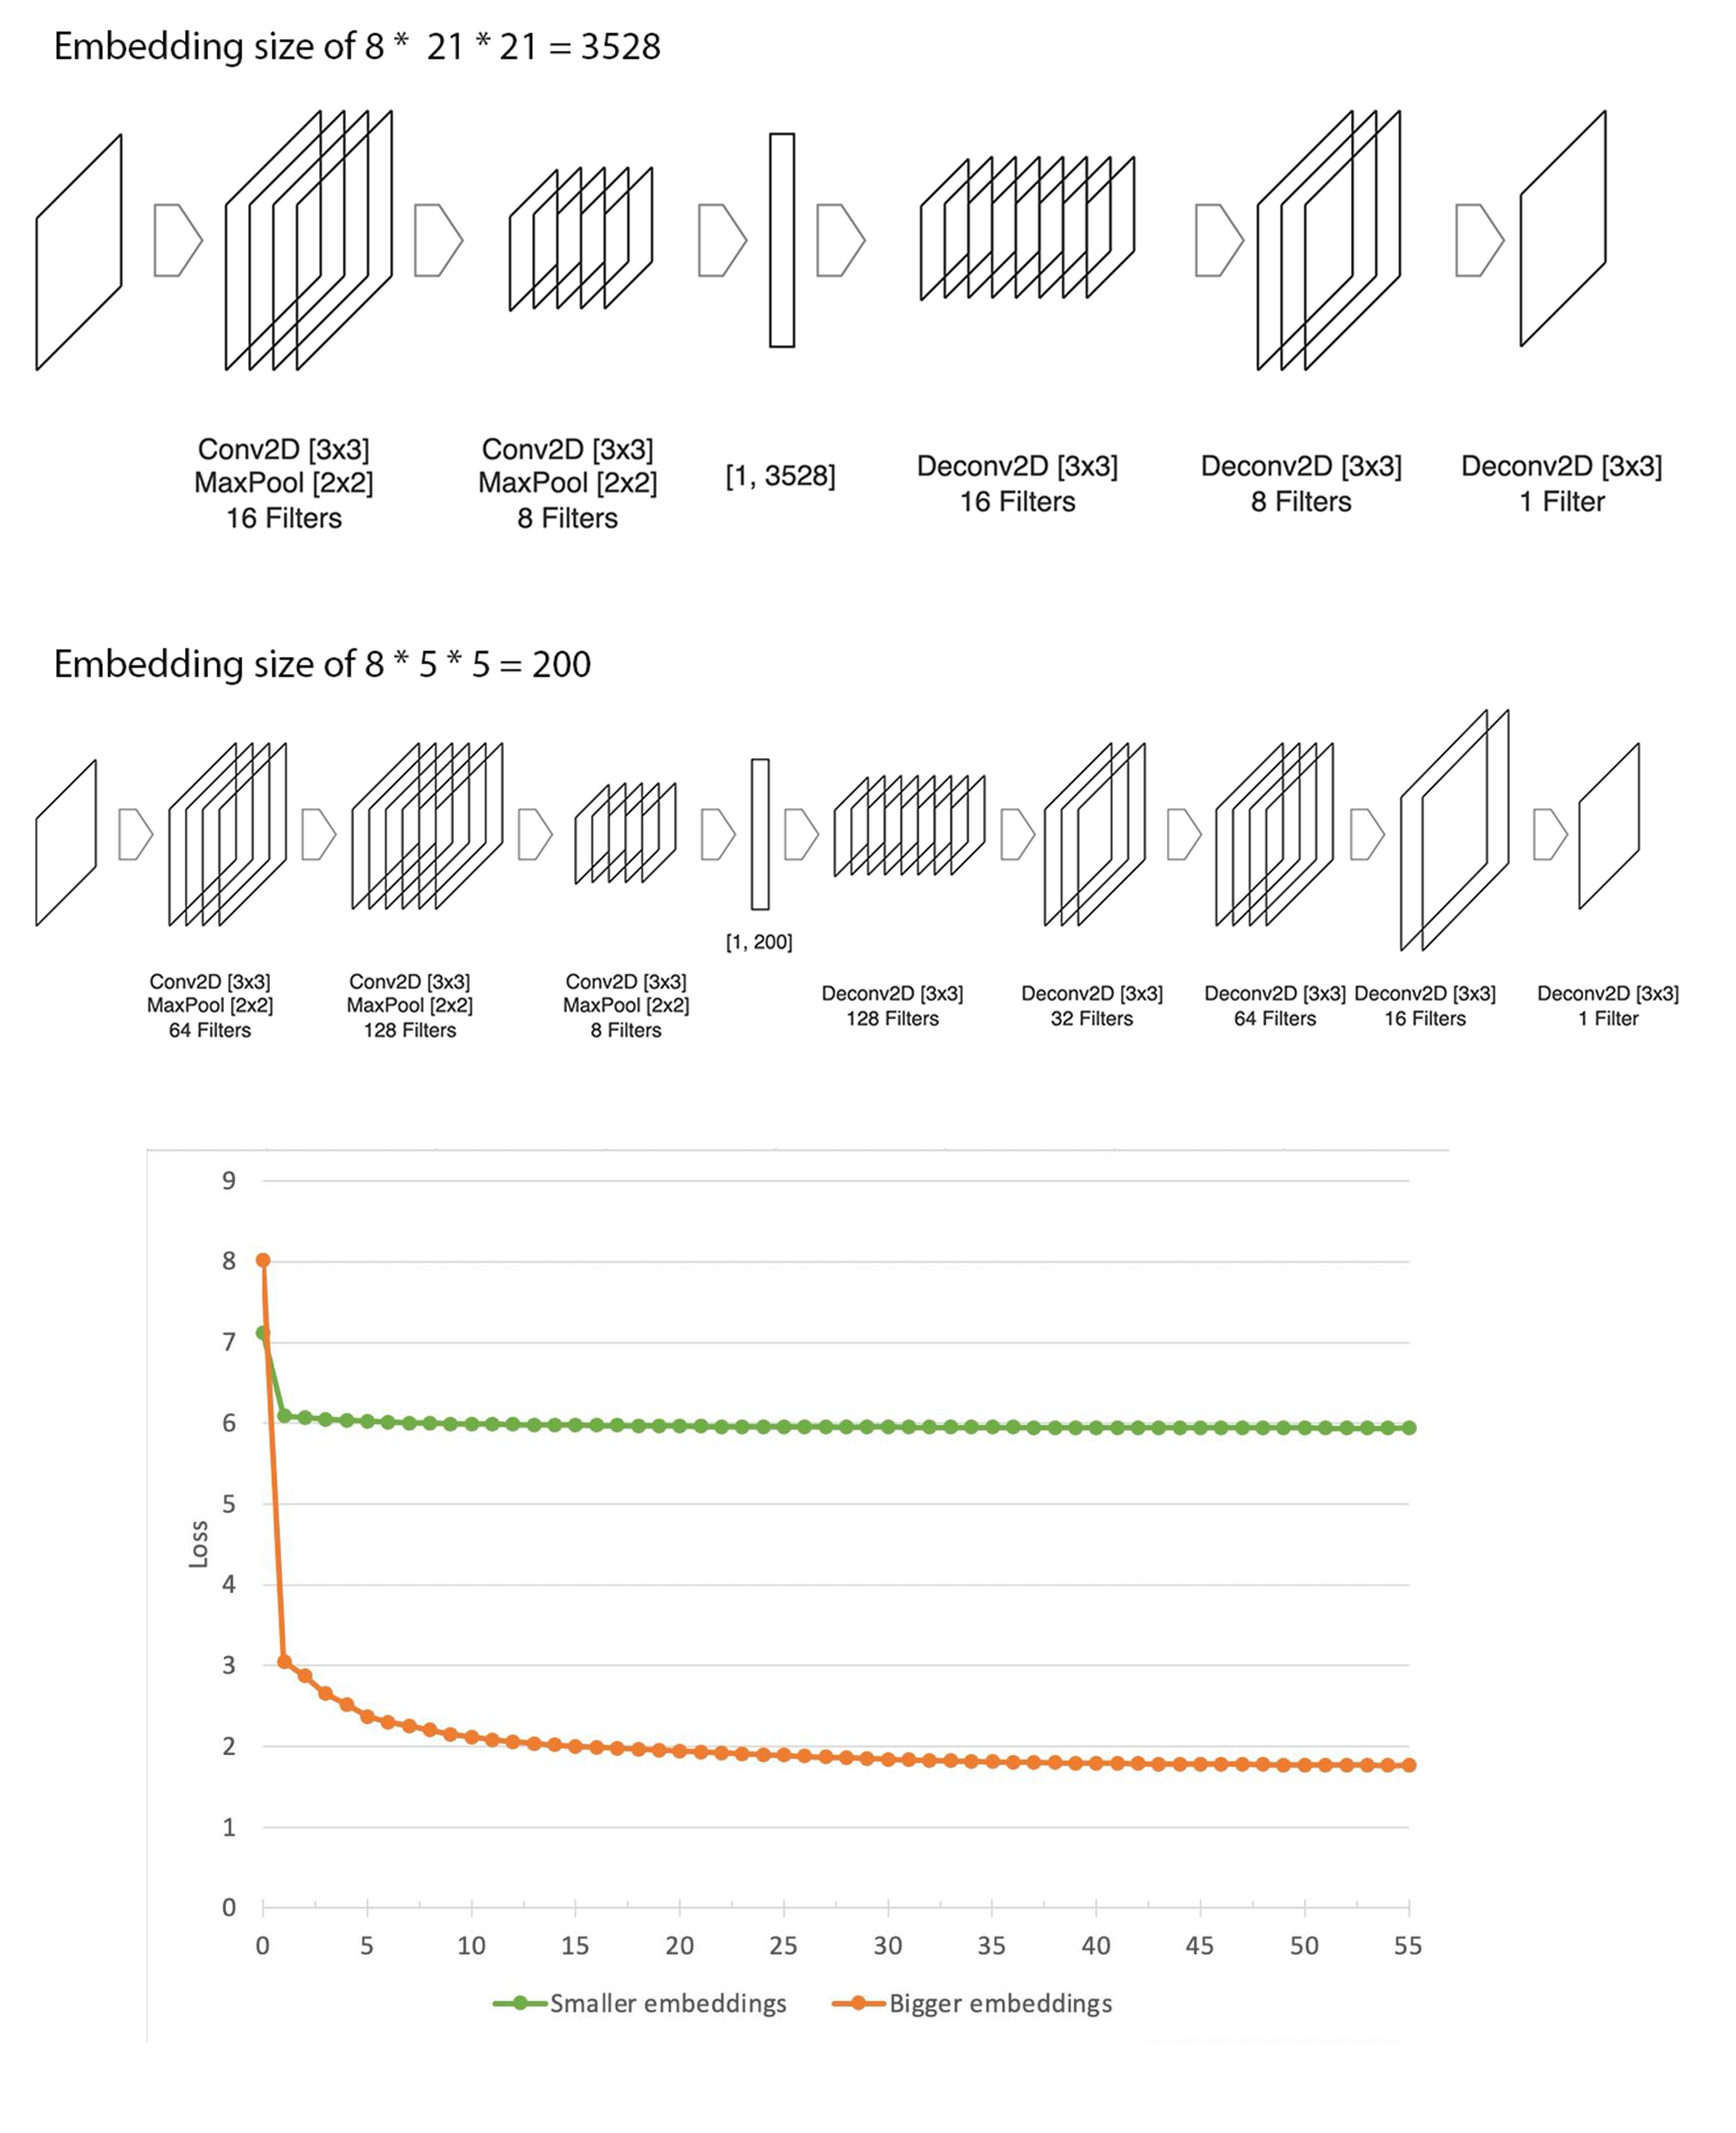
\includegraphics[width=\linewidth]{bilder/ae-embeddings/training-architectures.png}
		\caption{Architectures of two autoencoders and their training convergence}\label{fig:ae-training}
	\end{center}
\end{figure}

An autoencoder with embeddings of bigger size was able to achieve a lower loss as well as samples reconstructed from it were of a better quality (see Figure \ref{fig:ae-samples}). Clearly samples reconstruction will not be high resolution as there are no skip-connections in this architecture. However, this is also not needed, the only interest here would be to see whether autoencoder embeddings provide any insights on the data.
\begin{figure}[H]
	\begin{center}
		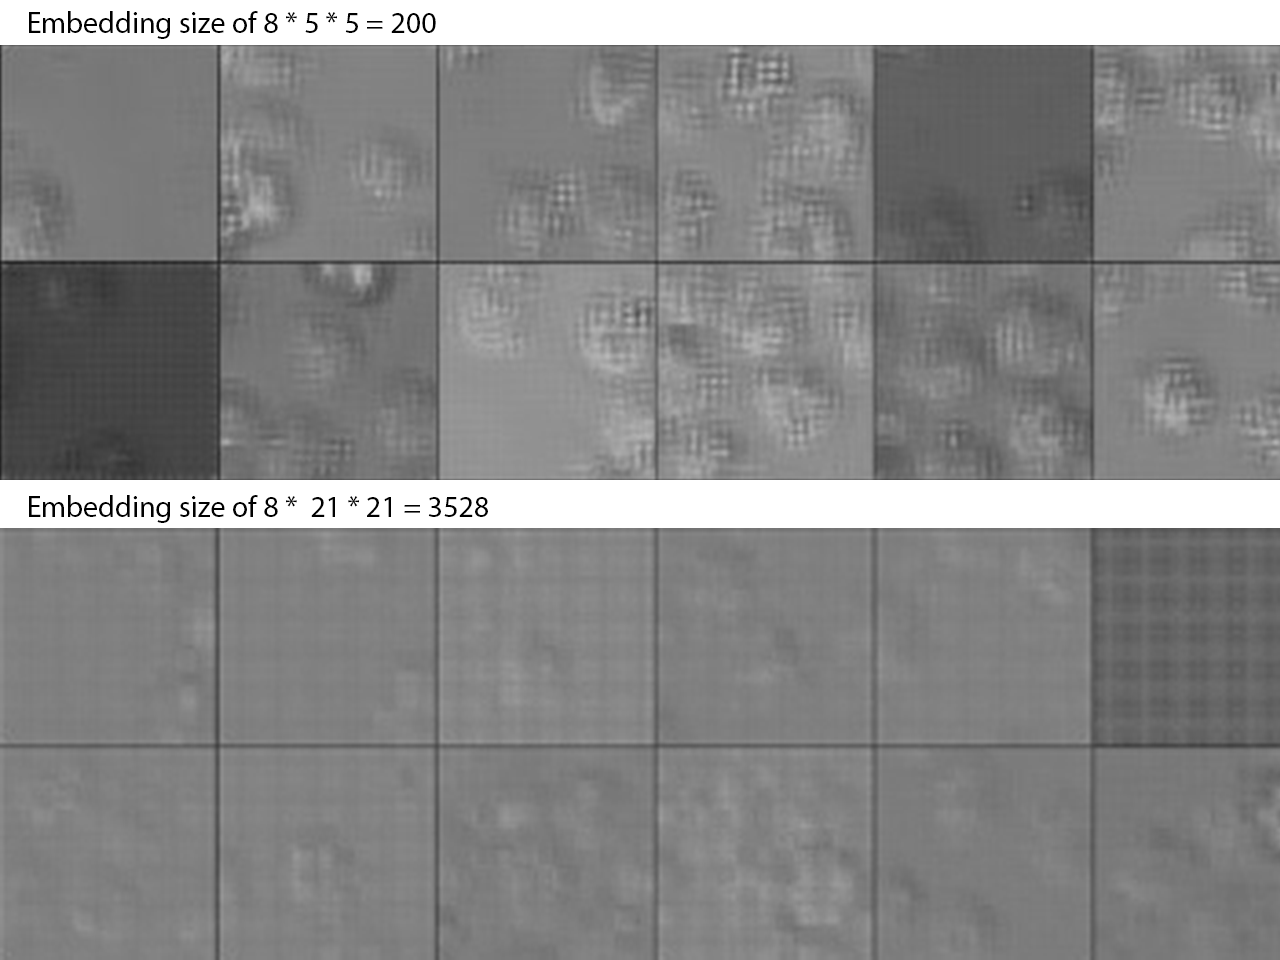
\includegraphics[width=0.5\linewidth]{bilder/ae-embeddings/ae-samples.png}
		\caption{Samples drawn from the trained autoencoder}
		\label{fig:ae-samples}
	\end{center}
\end{figure}

Since an autoencoder with bigger embeddings size seem to be able to reconstruct crops much better we have proceeded with its achtitecture. Embeddings were projected into a 2-dimensional space using first PCA with 10 components and then applying UMAP on PCA's projections. The results of such projection is presented in Figure \ref{fig:ae-pca-umap-clustered}. There are two clear clusters present: on the left are presented projections from earlier epoch and on the right after the model has converged. Embeddings separate clearly into two clusters throughout the training.

\begin{figure}[htb]
	\begin{center}
		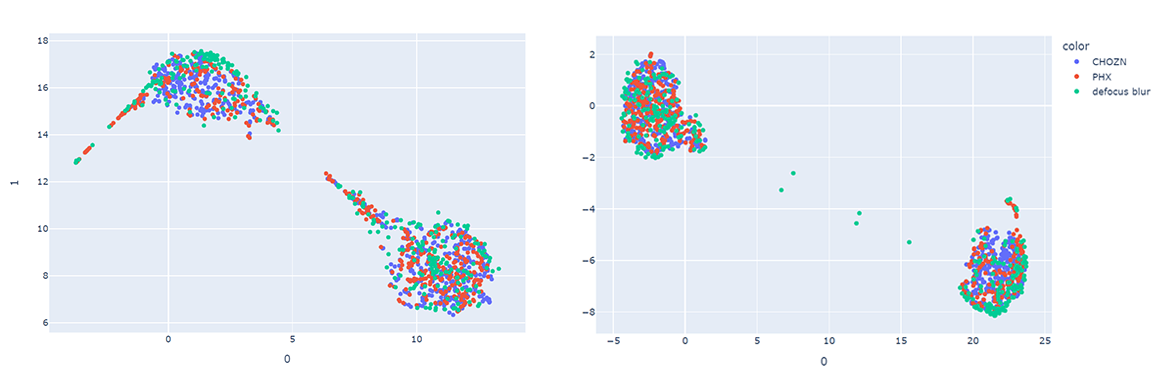
\includegraphics[width=0.8\linewidth]{bilder/ae-embeddings/pca-umap-clusters.png}
		\caption{Autoencoder embeddings after applying PCA with 10 components and UMAP afterwards. Earlier epoch VS later epoch}\label{fig:ae-pca-umap-clustered}
	\end{center}
\end{figure}

However these two clusters are base neither on cell phenotype nor on input corruption. All points of both phenotypd as well as corruptions seem to be equally mixed between two custers. By looking at the images correpondin to each of the clusters it soon became clear that the main difference between them is their brightness level. To prove this theory distirbutions of average image intensity for both clusters are presented in Figure \ref{fig:ae-brighter-darker}. It is clear tha from the violin plots that the distribution of crops on the left has a much lower brightness level than crops from the distribution on the right.
%\begin{figure}[htb]
%	\begin{center}
%		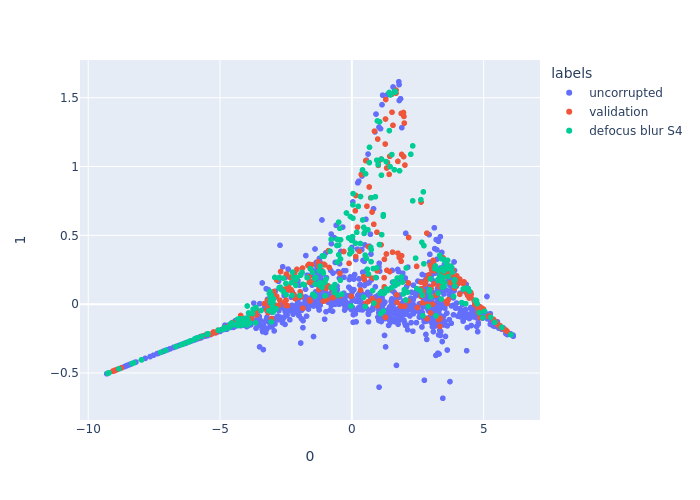
\includegraphics[width=0.5\linewidth]{bilder/ae-embeddings/pacmap.png}
%		\caption{PacMAP does not provide information on the coruption}\label{fig:ae-pacmap}
%	\end{center}
%\end{figure}

\begin{figure}[H]
	\begin{center}
		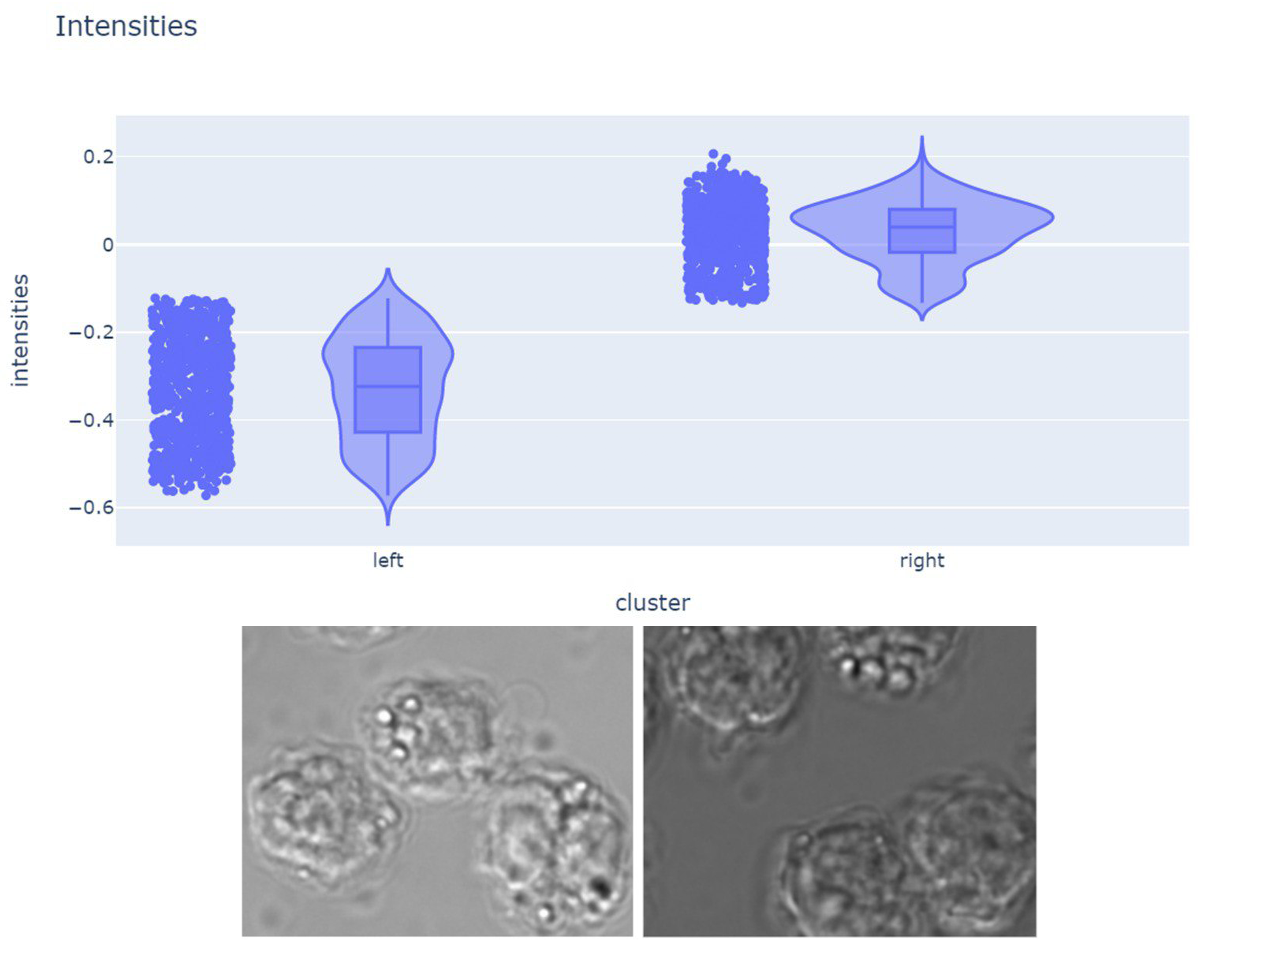
\includegraphics[width=0.5\linewidth]{bilder/ae-embeddings/brighter-darker.png}
		\caption{What do two UMAP clusters represent}
		\label{fig:ae-brighter-darker}
	\end{center}
\end{figure}

Since an autoencoder picks up on this difference within the crops it is worth trying to normalize crops the brightness across all crops. However this is not a trivial task as images have different cell density of them. That is why images that contained primarily background pixel will always be darker than the ones that contain enough of foreground. We suggest to filter the crops based on amount of cells critea (which can be done using GFP model that can detect cells present in DIC) and normalize them afterwards. Retraining autoencoder on new training data might provide more insights when difference in brightness will be gone.

It is also clear why autoencoder embeddings do not provide any clustering for corrupted crops. Corruption severities neither really change the image semantics nor they are significantly different visually (see defocus blur in \ref{fig:artificial-corruptions}). Therefore they do not alter the ability of an autoencoder to restore input correctly. In contrast, UNet predictions do suffer significantly for severy corruption levels, its predictions strongly changes --- outline of the organelle becomes more blurry, additional shine appears in fluprescence prediction. These changes happen not only during the decoding part, but they also might bring unsual values in the embedding representation. Therefore when UNet embeddings have more information on the "trustworthiness" of predictions. That is why for intance when defocus corruptions are used as training augmentations, drift detection for the model trained with these corruptions stops alarming about the drift, although it did for the model, which did not have these augmentations present. This happens simply because models predictions suffer and start to look different, which triggers a "drift alarm".